\documentclass[14pt]{extarticle}
\usepackage{amsmath}
\usepackage{amssymb}
\usepackage{tikz}
%\usetikzlibrary{calc}
\usetikzlibrary{trees}
\usepackage{hyperref}
\usepackage{graphicx}
\graphicspath{ {../../chap08/} }
\usepackage[top=0.75in, bottom=0.75in, left=0.75in, right=0.75in]{geometry}
\newcommand*{\Scale}[2][4]{\scalebox{#1}{\ensuremath{#2}}}%
\usepackage[shortlabels]{enumitem}
\usepackage[most]{tcolorbox}
\definecolor{bg}{RGB}{255,249,227}
% \usepackage{showframe}
\title{\vspace{-5ex}Math 208 Section 8.1, 8.2}
\date{\vspace{-10ex}}
\usepackage{multicol}
\setlength{\columnsep}{1cm}


\begin{document}
\maketitle		
\section*{Homework, Reading, and Other}
\begin{itemize}
	\item Section 7.2
	\item Section 7.3, 7.4
	\item Section 8.1, 8.2
\end{itemize}

\section*{Goals}
\begin{itemize}
	\item Understand and derive sample space and events from a statement
	\item Assign simple event probabilities
	\item Calculate compound probabilities
	\item Recognize and calculate union, intersection, and complement probabilities
	\item Relate odds to probabilities and be able to convert.
\end{itemize}

\section*{Probability}
Do you want to win at gambling or any games of chance? Then pay close attention to this chapter. Probability started as a way to understand (and improve odds) in gambling, however, it is now an immensely useful branch of mathematics with applications in practically every field.
\\\\
Probability is critical to understanding risk management, to diversification of investment portfolios, to designing a health care system, to creating plans for retirement, to assessing the risk vs reward for many business decisions, and numerous other applications.

\section*{8.1 Sample Space, Events, and Probability}
In probability theory, an experiment or trial is any procedure that can be infinitely repeated and has a well-defined set of possible outcomes, known as the sample space. An experiment is said to be random if it has more than one possible outcome. For purposes of this section, all experiments are considered random.
\\\\
\textit{Sample Space}, denoted by $S$, is the set all of the possible outcomes of an experiment. An \textit{Event}, denoted by $E$, is the actual outcome of the experiment. An event is always a subset of the sample space.

\subsection{Examples for Sample Space and Events}
Sample Space:
\begin{itemize}
	\item Roll a die: $S=\{1,2,3,4,5,6\}$
	\item Flip a coin twice: $S=\{HH,HT,TH, TT\}$
\end{itemize}
Simple Event:
\begin{itemize}
	\item Roll a 4: $E=\{4\}$
	\item Flip a coin twice and get heads and then tails: $E=\{HT\}$
\end{itemize}
Compound Event:
\begin{itemize}
	\item Roll an even die: $E=\{2,4,6\}$
	\item Flip a coin twice and get more at least 1 heads: $E=\{HH,HT,TH\}$
\end{itemize}
\vspace{5ex}
\textbf{Sample space for rolling two dice}: $S$ is the set of all ordered pairs in the figure.\\
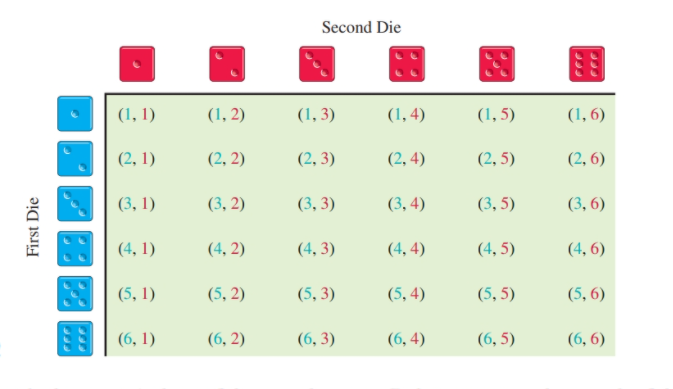
\includegraphics[width=0.9\linewidth]{8-1-5}
\begin{itemize}
	\item What is the event that a sum of 7 is rolled?
	\item $E = \{(6,1), (5,2),(4,3),(3,4),(2,5),(1,6)\}$
	\item What is the event that the sum $<4$?
	\item $E=\{(1,1),(1,2),(2,1)\}$
\end{itemize}

\subsection{Simple Event Probabilities}
\begin{tcolorbox}[enhanced jigsaw,colback=bg,boxrule=0pt,arc=0pt] 
	Given a sample space of $S = \{e_1, e_2, \cdots, e_n\}$ with $n$ simple events. The probability of event $e_i$ is $\mathbf{P(e_i)}$. $P(e_i)$ is subject to two conditions:
	\begin{enumerate}
		\item $P(e_i)$ is between $0$ and $1$, i.e.:
		\begin{align*}
			0 \leq P(e_i) \leq 1
		\end{align*}
		\item The sum of the probabilities of all simple events equals 1, i.e,:
		\begin{align*}
			P(e_1) + P(e_2) + \cdots + P(e_n) = 1
		\end{align*}
	\end{enumerate}
	Any probabilities that satisfy Conditions 1 and 2 are acceptable.
\end{tcolorbox}

\begin{tcolorbox}[enhanced jigsaw,colback=bg,boxrule=0pt,arc=0pt] 
	\textbf{Theorem: Assigning probability under the equally likely assumption} \\\\
	If we assume that each simple event in a sample space S is as likely to occur as any other, then the probability of an arbitrary event E in S is given by
	\begin{align*}
		P(E) = \frac{\text{number of elements in E}}{\text{number of elements in S}} = 
		\frac{n(E)}{n(S)}
	\end{align*}
\end{tcolorbox}


% Set the overall layout of the tree
\tikzstyle{level 1}=[level distance=3.5cm, sibling distance=3.0cm]
\tikzstyle{level 2}=[level distance=3.5cm, sibling distance=1cm]
% Define styles for bags and leafs
\tikzstyle{bag} = [text width=4em, text centered]
\tikzstyle{end} = [circle, minimum width=3pt,fill, inner sep=0pt]
\textbf{Sample space and probabilities for FAIR flipping a coin twice}\\
\begin{tikzpicture}[grow=right, sloped]
	\node[bag] {Start}
	child {
		node[bag] {T}        
		child {
			node[end, label=right:
			{T $\to$ combined event TT $p=\frac{1}{4}$}] {}
		}
		child {
			node[end, label=right:
			{H$\to$ combined event HT $p=\frac{1}{4}$}] {}
		}
	}
	child {
		node[bag] {H}        
		child {
			node[end, label=right:
			{T$\to$ combined event HT $p=\frac{1}{4}$}] {}
		}
		child {
			node[end, label=right:
			{H$\to$ combined event HH $p=\frac{1}{4}$}] {}
		}
	};
\end{tikzpicture}
\begin{itemize}
	\item What is the probability of flipping a head on one flip?
	\item $P(H) = 1/2$
	\item What is the probability of flipping a head or a tail on one flip?
	\item $P(H \text{ or } T) = P(H) + P(T) = 1/2+1/2 = 1$
	\item What is the event two of the same were flipped on two flips? $P(E)$?
	\item $E = \{HH, TT\}$
	\item $P(E) = 1/4 + 1/4 = 1/2$
\end{itemize}

\subsubsection*{Assignment from direct experiment}
If a coin were flipped 10,000 times, we would expect heads to turn up about 5,000 times. Likely, the results differed from exactly 5,000 but we would not suspect the coin to be unfair unless there was consistent and substantial difference from 5,000.
\\\\ 
Suppose the results showed 3,750 heads out of 10,000 flips. Now, we suspect that the coin is not fair and may decide to assign probabilities as follows:
\begin{align*}
	&P(H) = \frac{3750}{10000}=0.375 & P(T) = \frac{6250}{10000} =0.625&
\end{align*}
This assignment would be acceptable and reasonable. 

\subsection{Probability of Events}
\begin{tcolorbox}[enhanced jigsaw,colback=bg,boxrule=0pt,arc=0pt] 
	\begin{enumerate}
		\item If $E=\emptyset$, the empty set, then $P(E)=0$.
		\item If E is a simple event, then $P(E)$ is assigned as above.
		\item If E is a compound event, then $P(E)$ is the sum of its simple events.
		\item If $E=S$, the sample space, then $P(E)=1$.
	\end{enumerate}
\end{tcolorbox}


\section*{7.4 Permutations and Combinations}
We start this section by defining a mathematical operation called factorial. This might look similar to what we have just done in the Multiplication Principle.
\begin{tcolorbox}[enhanced jigsaw,colback=bg,boxrule=0pt,arc=0pt] 
	\textbf{Definition Factorial}:
	For any natural number $n$, 
	\begin{align*}
		&n! = n(n – 1)(n – 2)*\cdots*2*1   \\
		\\
		&0! = 1 \\
		\\
		&n! = n(n – 1)!
	\end{align*}
\end{tcolorbox}
\subsection{Factorial Examples}
\begin{align*}
	4! &= 4*3*2*1 = 24 \\\\
	\frac{9!}{8!} &= \frac{9*8!}{8!} = 9 \\\\
	\frac{16!}{13!} &= \frac{16*15*14*13!}{13!}= 16*15*14 = 3360 \\\\
	\frac{32!}{4!31!} &= \frac{32*31!}{0!31!}= \frac{32}{1} = 32
\end{align*}


\subsection{Permutations}
Say that we start with 5 shapes, $\Diamond, \Box, \bigcirc, \bigtriangleup, \cap$. How many different ways can theses shapes be arranged? It should follow that the number of ways is $5*4*3*2*1 = 5! = 120$. Now let's say that we have the same 4 shapes but are only interested in using 2 of them? 
\\\\
A permutation of a set of $n$ distinct objects taken $r$ at a time without repetition is an arrangement of $r$ of the $n$ objects in a specific order.
\\\\
In arranging our shapes, that means there are $5*4$ permutations. Denote the permutations as, $_nP_r$, then
\begin{align*}
	_nP_r = 5*4 = \frac{5*4*3*2*1}{3*2*1} = \frac{5!}{3!}
\end{align*}
\begin{tcolorbox}[enhanced jigsaw,colback=bg,boxrule=0pt,arc=0pt] 
	\textbf{Permutations}: The number of permutations of n distinct objects taken r at a time without repetition is given by
	\begin{align*}
		_nP_r &= n(n-1)(n-2)* \cdots *(n-r+1)\\
		&\text{or} \\
		_nP_r &= \frac{n!}{(n-r)!}
	\end{align*}
\end{tcolorbox}

\subsubsection{Example}
Find the number of permutations of 30 objects taken 4 at a time. Find this using the formulas and then using the permutation key on your calculator.
\begin{align*}
	_{30}P_4 &= 30(30-1)(30-2)(30-3) = 30*29*28*27 = 657,720 \\
	_{30}P_4 &= \frac{30!}{(30-4)!} = \frac{30!}{(26)!} = 657,720
\end{align*}


\subsection{Combinations}
Starting with the same 5 shapes, $\Diamond, \Box, \bigcirc, \bigtriangleup, \cap$. How many different combinations of 2 can we choose? In this case, the order of the selection does not matter. For permutations, order matters but for combinations, order does not matter.
\\\\
A combination of a set of n distinct objects taken r at a time without repetition is an r-element subset of the set of n objects. The arrangement of the elements in the subset does not matter. Denote this by $_{n}C_r$.

\begin{tcolorbox}[enhanced jigsaw,colback=bg,boxrule=0pt,arc=0pt] 
	\textbf{Combinations}:  The number of combinations of n distinct objects taken r at a time without repetition is given by
	\begin{align*}
		_nC_r =&n\choose r\\
		&= \frac{_nP_r}{r!}\\
		&\text{or} \\
		&= \frac{n!}{r!(n-r)!} &0 \leq r \leq n
	\end{align*}
The above formula are developed in the book if you are interested.
\end{tcolorbox}

\subsubsection{Examples}
Choose 2 of 5 shapes. Find this using the formulas and then using the combination key on your calculator.
\begin{align*}
	_{5}C_2 &= \frac{_5P_2}{2!} = \frac{20}{2} = 10 \\
	_{5}C_2 &= \frac{5!}{2!(5-2)!} = \frac{5!}{2!(3)!} = 10
\end{align*}
\\\\
A company has 7 senior and 5 junior officers. It wants to form an ad hoc legislative committee.
\begin{enumerate}[A)]
	\item How many 4-officer committees with 1 senior officer and 3 junior officers can be formed?
	\begin{align*}
		_{7}C_1 * _{5}C_3 = 7*10=70
	\end{align*}
	\item How many 4-officer committees with 4 junior officers can be formed?
	\begin{align*}
		_{5}C_4 = 5
	\end{align*}
	\item How many 4-officer committees with at least 2 junior officers can be formed?
	\begin{align*}
		_{7}C_2 * _{5}C_2 +_{7}C_1*_{5}C_3 + _{5}C_4 = 21*10+7*10+5=285
	\end{align*}
\end{enumerate}



\noindent\rule{\textwidth}{1pt}
{\footnotesize Copyright (C) 2021 Garold Dalton --- Released under GNU General Public License v3.0}


\cleardoublepage


\end{document}
